\chapter{Introduction}
\section{Background and Motivation}
Robotic surface finishing, including polishing, sanding, grinding, and buffing, is a physically demanding and quality-sensitive manufacturing process. The final result depends not only on the nominal path of the robot but also on contact pressure, sliding velocity, dwell time, tool orientation, abrasive state, and local surface geometry. Conventional fixed-path automation can achieve high repeatability on structured parts, yet it is difficult to transfer to high-mix products containing large smooth regions, sharp boundaries, concave transitions, narrow features, and reflective hardware.

The dominant automation pipeline combines three-dimensional perception or CAD with explicit coverage planning and compliant control. A surface model provides normals, curvature, boundaries, and collision geometry; a planner generates a raster, iso-parametric, geodesic, or region-based trajectory; and a force, impedance, or admittance controller maintains contact. Recent work has improved uniform coverage, segmentation, contact-point switching, and manipulator feasibility~\cite{schneyer2023segmentation,tafuro2024autonomous,gong2025uniform,wang2025coverage,pusnik2025region}. These methods are effective on broad and continuously observable surfaces because product variation can be represented by a new CAD or mesh while reusing the same planning algorithm.

However, full-product polishing exposes two unresolved limitations. First, a path that covers a mathematical surface does not necessarily cover the surface with the physical tool. A polishing pad has a finite and deformable footprint. The path spacing must therefore depend on the effective tool width, overlap ratio, surface curvature, tool tilt, and boundary offset. The tool center point (TCP) is a point and has no width; throughout this thesis, the phrase \emph{tool width} refers to the effective contact footprint of the polishing tool. Second, geometric coverage does not guarantee uniform material removal because the actual pressure and sliding velocity vary during execution. According to the Preston relation, the local removal rate is approximately proportional to their product~\cite{preston1927theory}.

A third challenge occurs at edges, cutaways, narrow transitions, and hardware-adjacent regions. Modern geometric planners can introduce region-specific strategies and move the tool contact point, but their rule and parameter complexity grows with the number of local contact modes~\cite{schneyer2023segmentation}. In repair and reconditioning, the geometry is further combined with product-specific scratches, oxidation, loss of gloss, and wear. The desired approach direction, tool tilt, contact-force reduction, repeated short strokes, and termination time may be easier for a skilled operator to demonstrate than to specify through a universal analytical objective.

This thesis therefore proposes a hybrid architecture. Tool-footprint-aware full-coverage planning is used for the entire CAD surface and broad regular regions. Reinforcement learning optimizes the sliding velocity along the geometric path while the path and low-level admittance controller remain fixed. Force-aware imitation learning generates local pose--force trajectories for difficult segments. Finally, object-centric and predictive feature masking is introduced to reduce the influence of reflections, background clutter, and irrelevant image regions on the imitation-learning policy.

\begin{figure}[t]
    \centering
    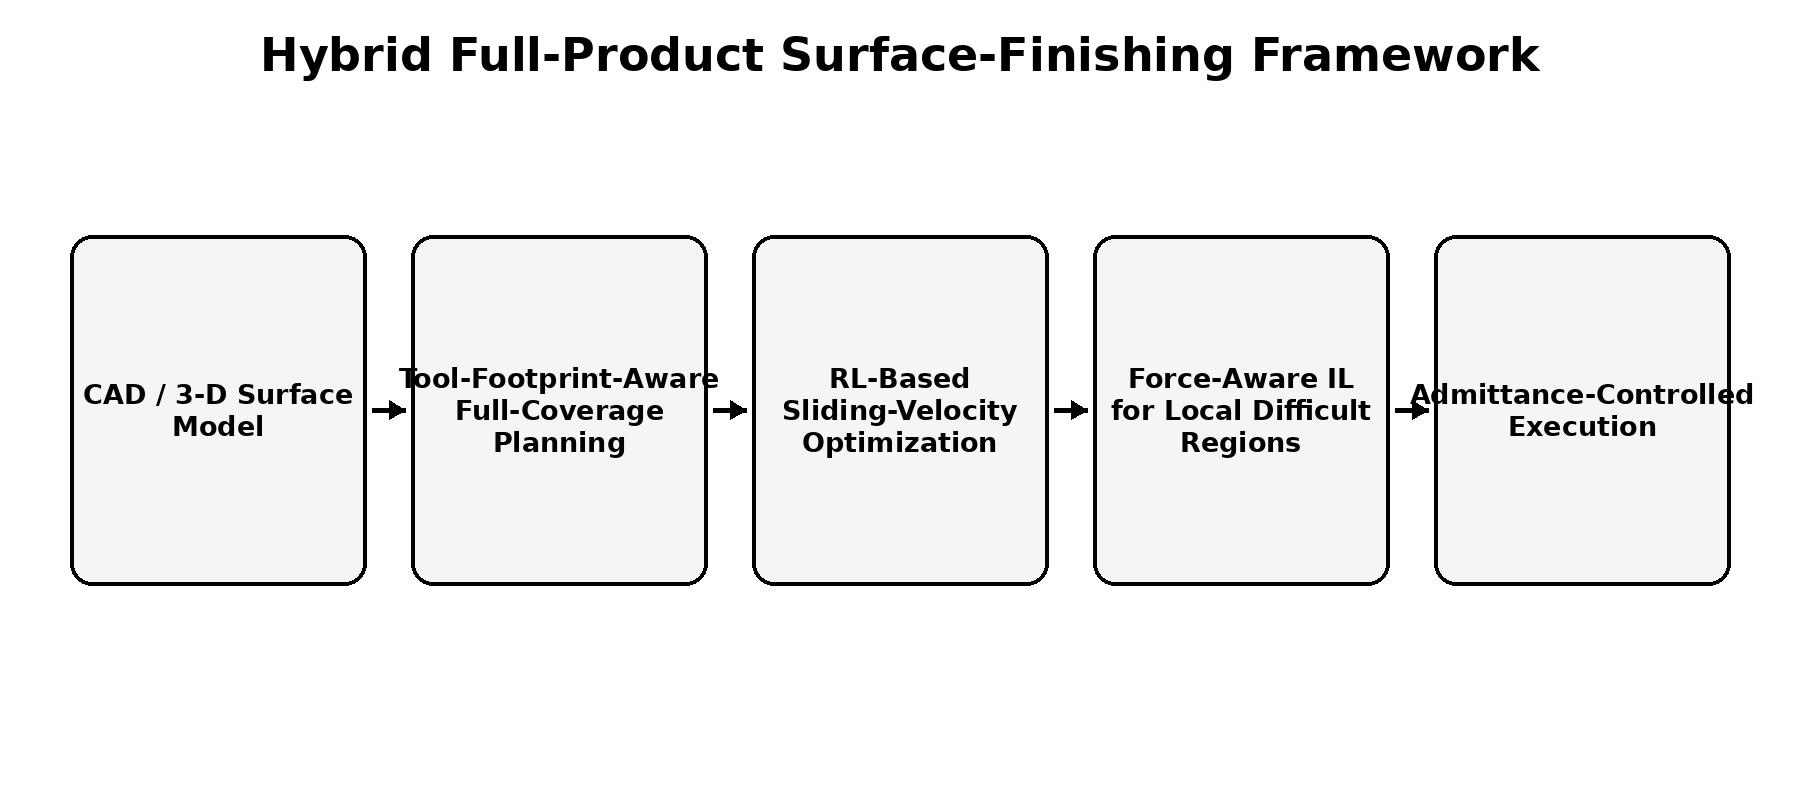
\includegraphics[width=0.98\textwidth]{./1.Introduction/figs/overall_framework.png}
    \caption{Overall structure of the proposed hybrid full-product surface-finishing framework.}
    \label{fig:overall_framework}
\end{figure}

\section{Related Works}
\subsection{Surface Reconstruction and Coverage Planning}
Scan-based robotic surface finishing has progressed from planar projection toward free-form surface reconstruction, segmentation, geodesic planning, and kinematics-aware optimization. Tafuro et al. studied planning from realistic industrial scans and emphasized incomplete reconstruction and abrupt curvature changes~\cite{tafuro2024autonomous}. Schneyer et al. segmented free-form surfaces and selected different finishing-disk contact points to improve access to concave regions~\cite{schneyer2023segmentation}. Gong et al. generated uniform coverage trajectories on equation-free mesh surfaces~\cite{gong2025uniform}, while recent planners exploit redundancy, region decomposition, and task-aware partitioning~\cite{wang2025coverage,pusnik2025region,yu2026fusion}.

These studies show that local feature coverage can be addressed geometrically when the workpiece and tool model are accurate. Nevertheless, every new contact mode may require a new region classifier, contact-point rule, clearance threshold, or trajectory topology. This thesis retains advanced geometric planning as a strong baseline but uses imitation learning where the desired strategy depends jointly on geometry, visual condition, and contact feedback.

\subsection{Material-Removal Optimization and Reinforcement Learning}
Coverage and removal uniformity are distinct. Recent polishing studies jointly consider force, position, and speed~\cite{adaptive2025force}, constant-pressure processing on curved surfaces~\cite{huang2025marble}, or data-driven material-removal estimation~\cite{darowski2025mrr}. Reinforcement learning has also been used to learn abrasive shape transitions or force-responsive finishing skills~\cite{hachimine2023grinding,wang2023adaptive}. In contrast, the proposed RL policy controls only a scalar path-progress rate above a fixed CAD path and admittance controller. This restricted action space is intended to improve safety, interpretability, and sim-to-real transfer.

\subsection{Force-Aware Imitation Learning}
Force-aware imitation learning has rapidly developed for contact-rich tasks. ForceMimic records force-motion demonstrations and predicts hybrid force-position parameters~\cite{liu2025forcemimic}. FoAR fuses RGB and high-frequency force/torque signals with a future-contact predictor~\cite{he2025foar}. DexForce computes force-informed actions from kinesthetic demonstrations~\cite{chen2025dexforce}, and Flow with the Force Field learns compliant flow-matching policies from demonstration-guided simulation data~\cite{li2026flowforce}. These methods establish that force is valuable in contact-rich policy learning, but they also prevent a broad novelty claim based only on force input or output. The contribution of this thesis is instead defined by selective local teaching, a continuous 9-D pose--force action chunk, direct integration with an admittance controller, and full-product coordination with global planning and RL process optimization.

\subsection{Object-Centric and Mask-Guided Policy Learning}
VIOLA constructs object-centric representations from general object proposals generated by a pretrained vision model and uses a transformer policy to attend to task-relevant visual factors~\cite{zhu2023viola}. Mask2Act predicts future masks of task-relevant objects as latent plans from action-free video and uses them to guide policy learning with limited robot action data~\cite{zhang2025mask2act}. Both methods are relevant to polishing, where bright reflections, background texture, and non-target hardware can dominate a conventional image encoder. Chapter~\ref{chap:feature_masking} adapts their ideas to a force-aware polishing policy.

\section{Research Objectives}
The objective is to develop and evaluate a modular framework with the following functions:
\begin{enumerate}
    \item generate a full-coverage path over an entire CAD surface using the effective polishing-tool footprint and overlap ratio;
    \item learn an adaptive sliding-velocity policy that reduces spatial variation of the Preston rate without directly controlling robot joints or the 6-D pose;
    \item learn local pose--force action chunks from expert demonstrations for edges and contact-sensitive regions;
    \item incorporate VIOLA-inspired region tokens and Mask2Act-inspired predictive mask plans into the force-aware IL framework;
    \item validate the complete framework on a guitar-scale object using coverage, removal, force, safety, efficiency, and generalization metrics.
\end{enumerate}

\section{Thesis Organization}
Chapter~2 defines the shared system interfaces and problem formulation. Chapter~3 presents tool-footprint-aware full-coverage path planning. Chapter~4 describes RL-based sliding-velocity optimization. Chapter~5 presents force-aware imitation learning. Chapter~6 proposes the feature-masking architecture. Chapter~7 defines the experimental design, and Chapter~8 concludes the thesis and outlines future work.
